\documentclass[../Relazione.tex]{subfiles}


\begin{document}
\section{Analisi pagine}
    \subsection{Homepage}
        \begin{figure}[!h]
            \centering
            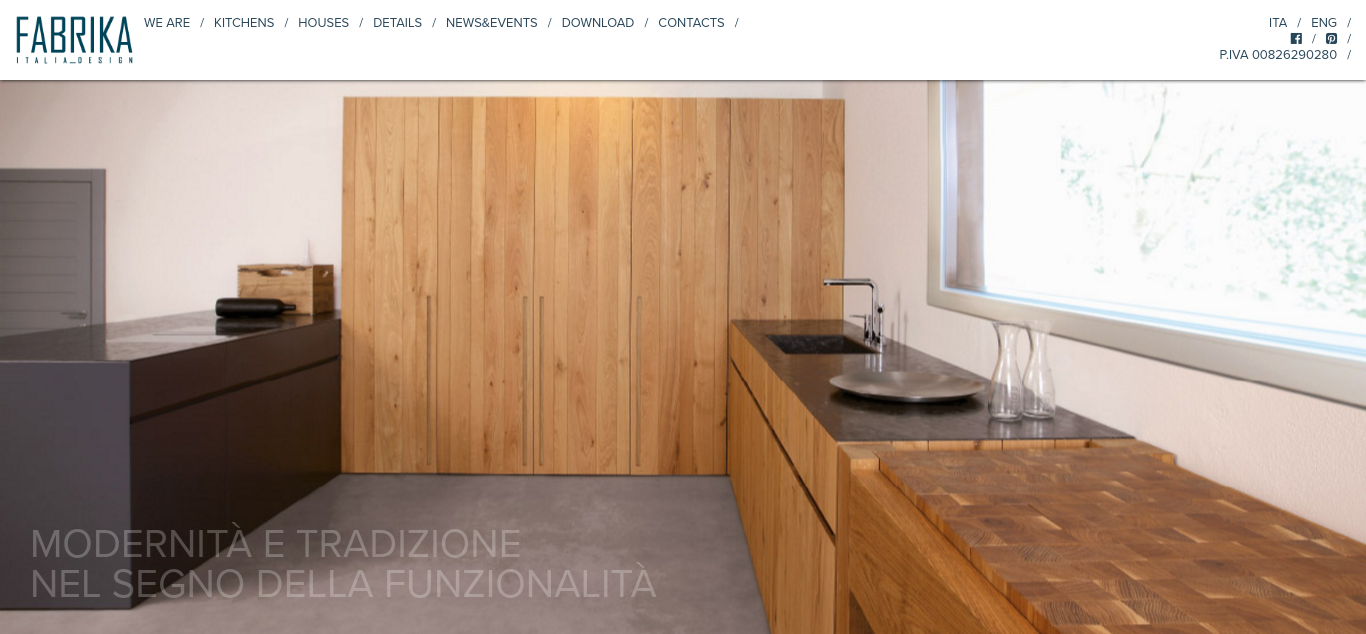
\includegraphics[width=\textwidth]{img/home.png}
            \caption{Homepage - home.png - (\url{http://www.fabrikaitaliadesign.it/}(2017/07/29))}
        \end{figure}
       
     
        \subsubsection{Assi fondamentali}
            \paragraph{Where}
            Di primo acchitto non è chiara la tipologia di prodotti che vende a causa dello slider che copre tutta la pagina con foto di case con dei loro prodotti, purtroppo non si capisce subito se l'azienda vende interni, pavimenti o per l'appunto arredi.
           

            \paragraph{Who}
            E’ presente in alto a sinistra il logo dell’azienda che lo gestisce, un punto focale di considerevole importanza per l’utente. Purtroppo però alla sua pressione il sito riporta solo alla home page e per avere più informazioni riguardo all'azienda bisogna premere sulla sezione "We Are" che solo a tentativi è possibile scoprire che è la sezione riguardo alla storia dell'azienda.
            I contatti quali pt.Iva e contati social sono nel posto sbagliato, dovrebbero essere sotto e non in alto a destra.

            \paragraph{Why}
            Il perchè scegliere questo sito non è molto chiaro dalla home, si intuisce solo ed esclusivamente dalla frase allegata ad ogni foto nello slider, questo non è una buona mossa per far capire all'utente il motivo per cui deve scegliere \name\ e non altri.
            Il "Why" lo si capisce solo visitando le sezioni "We Are", "Kitchen", "houses".

            \paragraph{What}
             Di primo acchitto non è subito comprensibile cosa propone.
            Lo si capisce successivamente a metà grazie dallo slider che mostra una serie di foto di ambienti con arredo con una frase significativa, quasi sempre una frase "filosofica" sul proprio lavoro.
            Lo si capisce completamente andando nella sezione "We Are" che spiega che fanno ma questo porta via tempo al visitatore. Sicuramente non bastano 31 secondi per capirlo.
            
            
           

            \paragraph{When}
            E' presente una sezione solo ed esclusivamente con le notizie dell'azienda e del mondo dell'arredamento complete di date e link alla notizia.
            
            \paragraph{How}
            L'indice delle informazioni che propone il sito è chiara ma è dubbia la differenza tra le sezioni "kitchen" e "Houses" perche sembrano molto simili ad uno primo sguardo.
           Purtroppo l'uso dell'inglese per i menù anche con lingua italiana inserita è molto malvista dagli utenti e questo può creare molto disorientamento.
           La barra di ricerca non è presente anche se per un sito vetrina di queste dimensioni non servirebbe a molto.

        \subsubsection{Altri fattori}
            Le sezioni non sono ben divise perchè la sezione "Kitchen" che mostra foto di cucine da loro prodotte non è poi così diversa dalla sezione "Houses" che mostra prodotti in tutto lo spazio di una casa.
            I punti del menù sono in inglese anche se l'utente sceglie la lingua italiana e questo può portar sia nervosismo sia, nei peggiori casi, disorientamento per l'utente che non sa bene la lingua inglese.
            Lo slider prende tutta la pagina e sopratutto non da molte informazioni occupando tutto lo spazio di maggior attenzione da parte del visitatore.

    \subsection{Pagine interne in generale}
        \subsubsection{Assi obbligatori}
            \paragraph{Where}
E’ un asse opzionale ma è consigliatissimo poiché se assente obbliga l’utente a navigare senza sapere con precisione dove si trova, inoltre con il fenomeno del deep linking, dai motori di ricerca, serve un riferimento.
In questo caso il sito non offre nessun breadcamp nel sito, l'unica informazione lo da l'url della pagina.
            \paragraph{Why}
Molto presente nelle sezioni interne ma  non esattamente nel punto di massima attenzione da parte di un utente.
            \paragraph{When}
E' sempre possibile risalire alla pagina delle novità attraverso il menu.
            \paragraph{How}
Rimane inalterato il layout a schede già presente nella homepage. 
        
        \subsubsection{Assi opzionali}

            \paragraph{How}
Continua ad essere presente il logo in alto ma persistono le problematiche relative all’assenza di una descrizione riguardante l’azienda che sono rimandate in alto a destra per pochi contatti oppure in un altra sezione per la storia dell' azienda
            \paragraph{What}
            L'asse è maggiormente espresso dalla lista delle sezioni del sito.

        \subsection{ Altre considerazioni}
        In ogni sezione(escusa l'Home) si ha in codice dell' elemento scelto in caratteri cubitali e in carattere nettamente più piccolo la descrizione, questa scelta può portare sia disorientamento sia perdita di informazioni.
       \\
       Foto molto grandi ma capibile visto il ruolo del sito, cioè dimostrare i propri prodotti. Bene le foto cliccabili e la sezione News ben organizzata.
      
\newpage
    \subsection{Pagina We Are}
        \begin{figure}[H]
            \centering
            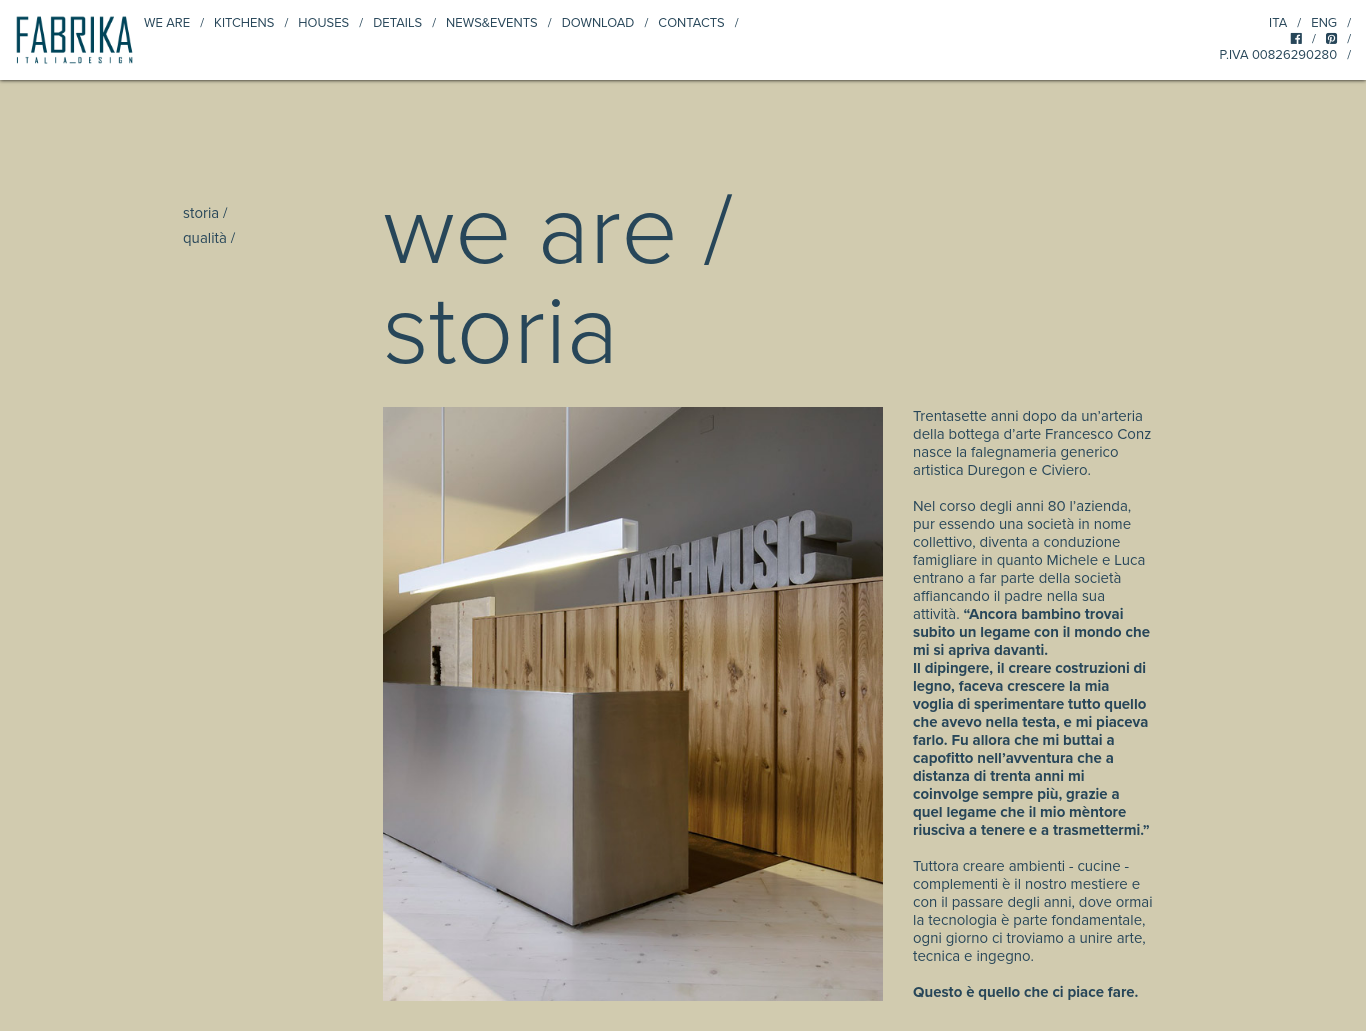
\includegraphics[width=\textwidth]{img/WeAre.png}
            \caption{Pagina We Are - WeAre.png - (\url{http://www.fabrikaitaliadesign.it/fabrika_italia_design_storia.html}(2017/06/29))}
        \end{figure}
       La scritta we are / storia, come detto in precedenza, è troppo grande e fa perdere molto spazio per informazioni più utili infatti per visualizzare tutta la pagina servono quasi 2 scroll.
       L'immagine è troppo grande e fa perdere spazio ad una pagina dove le informazioni sono più importanti delle foto. Metà delle informazioni presenti in questa pagina sono ti tipo "politichese", buona solo l'ultima parte che danno l'informativa del "Why" ma solo una piccolissima percentuale degli utenti arrivano a leggere fino a li.
      Male l'url che essendo troppo lungo in mobile può essere tagliato eliminando l'unita informazione dell'asse where.

    \subsection{Pagina Details}
        \begin{figure}[H]
            \centering
            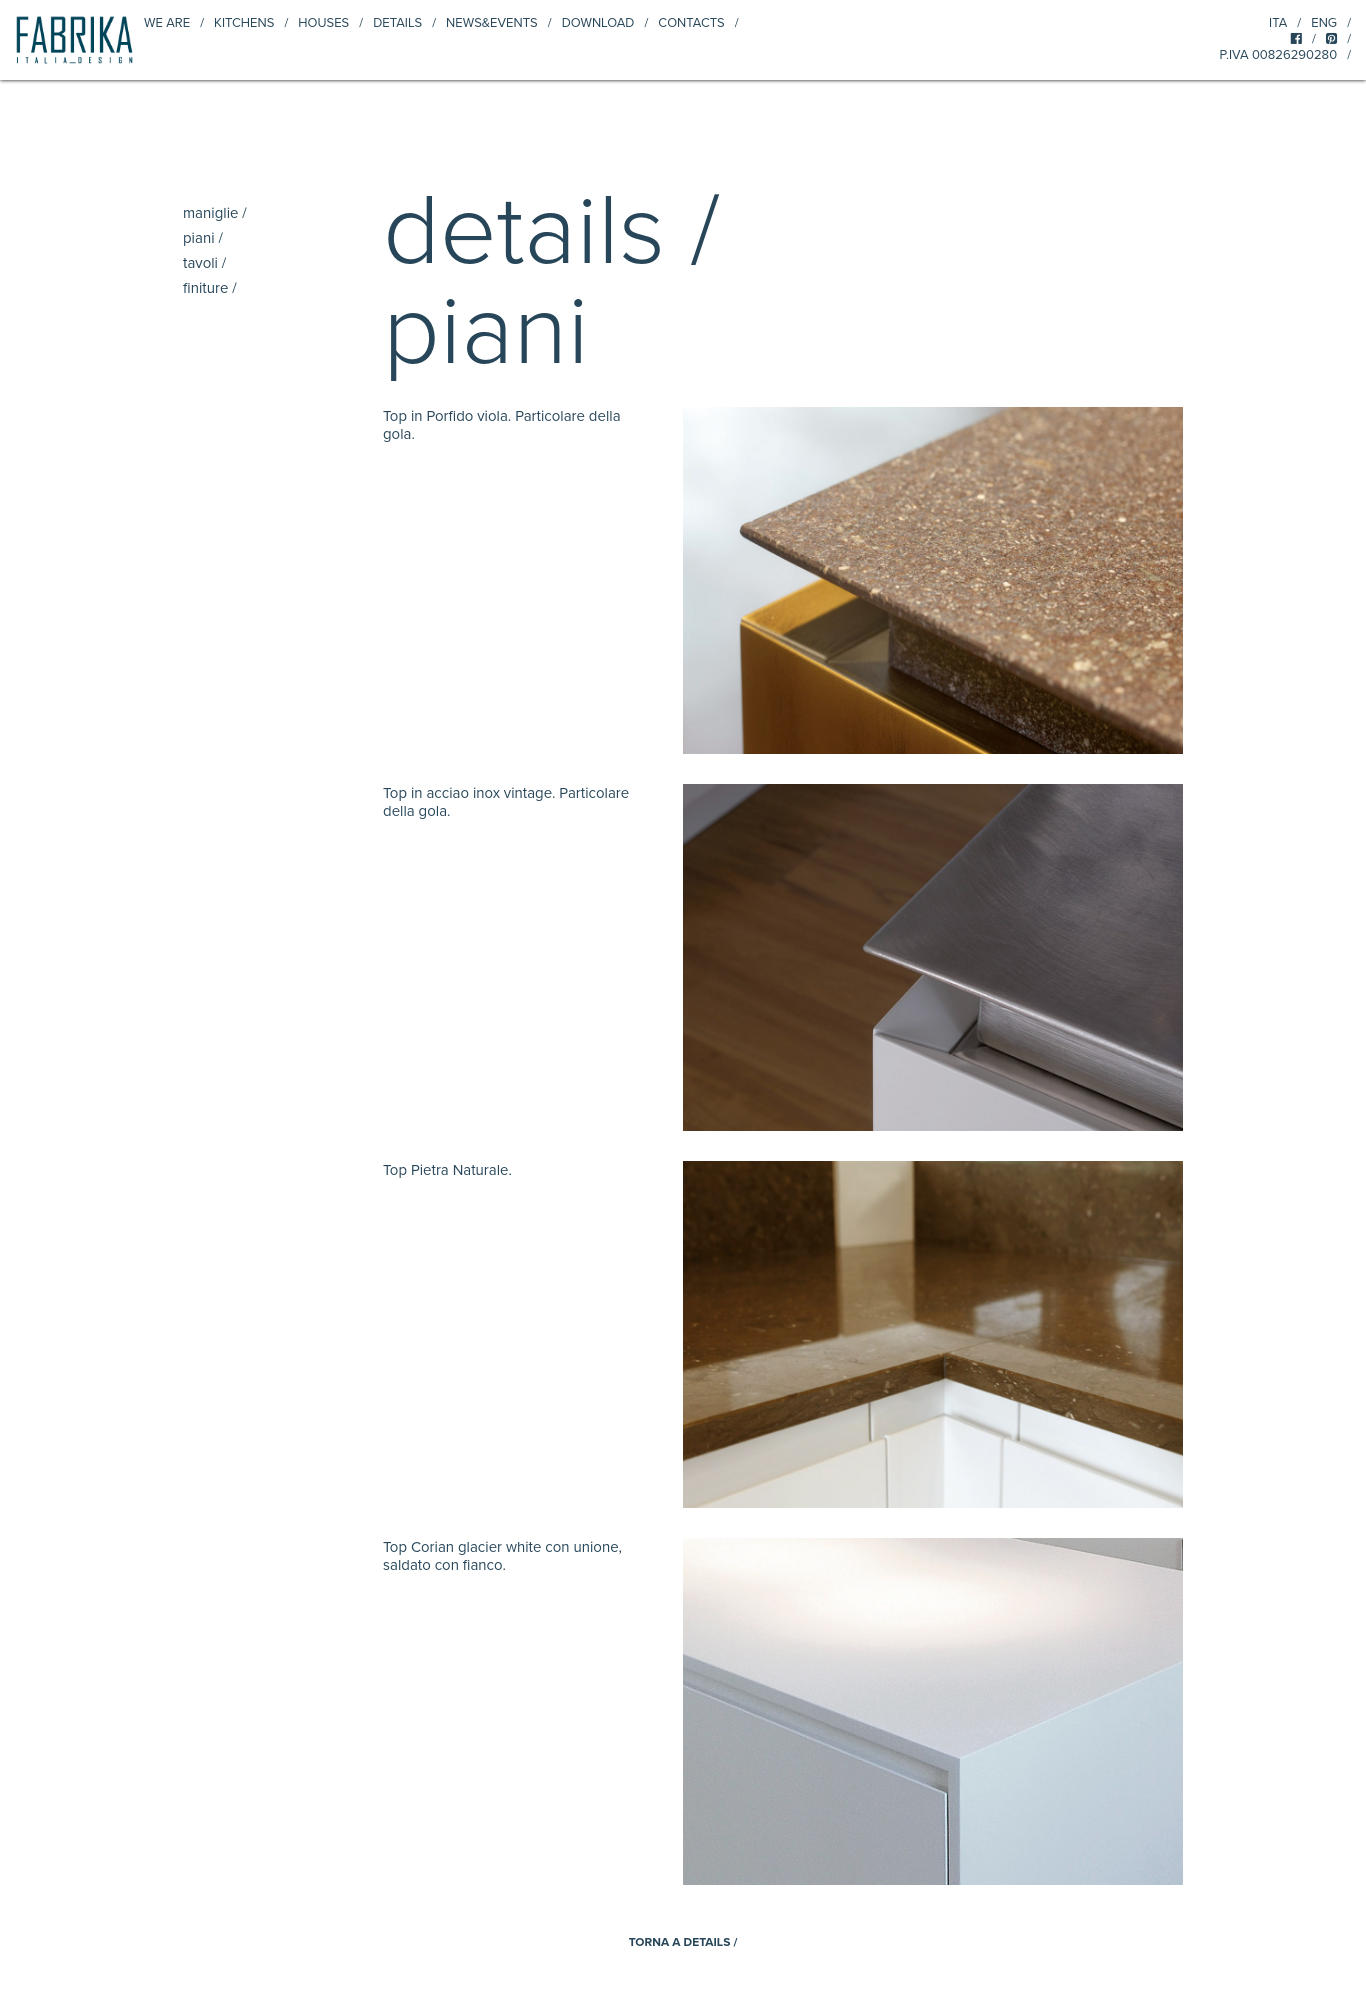
\includegraphics[width=\textwidth]{img/Details.png}
            \caption{Pagina Details - details.png - (\url{http://www.fabrikaitaliadesign.it/piani.html}(2017/06/29))}
        \end{figure}
        Tutto troppo grande infatti senza usar nessuno scroll non si riesce ad avere nessuna informazione aggiuntiva riguardo all'azienda, va bene che il sito è un sito copertina e deve mostrare anche molte foto ma qui non si riesce a capire il perchè quei siano dettagli di nota importanza.
        Bene le immagini cliccabili ma purtroppo non è possibile lo zoom.\\
        Breadcamp inesistente e l'url non rispecchia totalmente la posizione della pagina.\\
        Bene a fondo pagina(sarebbe stata meglio ad inizio) la possibilità di tornare alla root della pagina.

    \subsection{Pagina News}
        \begin{figure}[H]
            \centering
            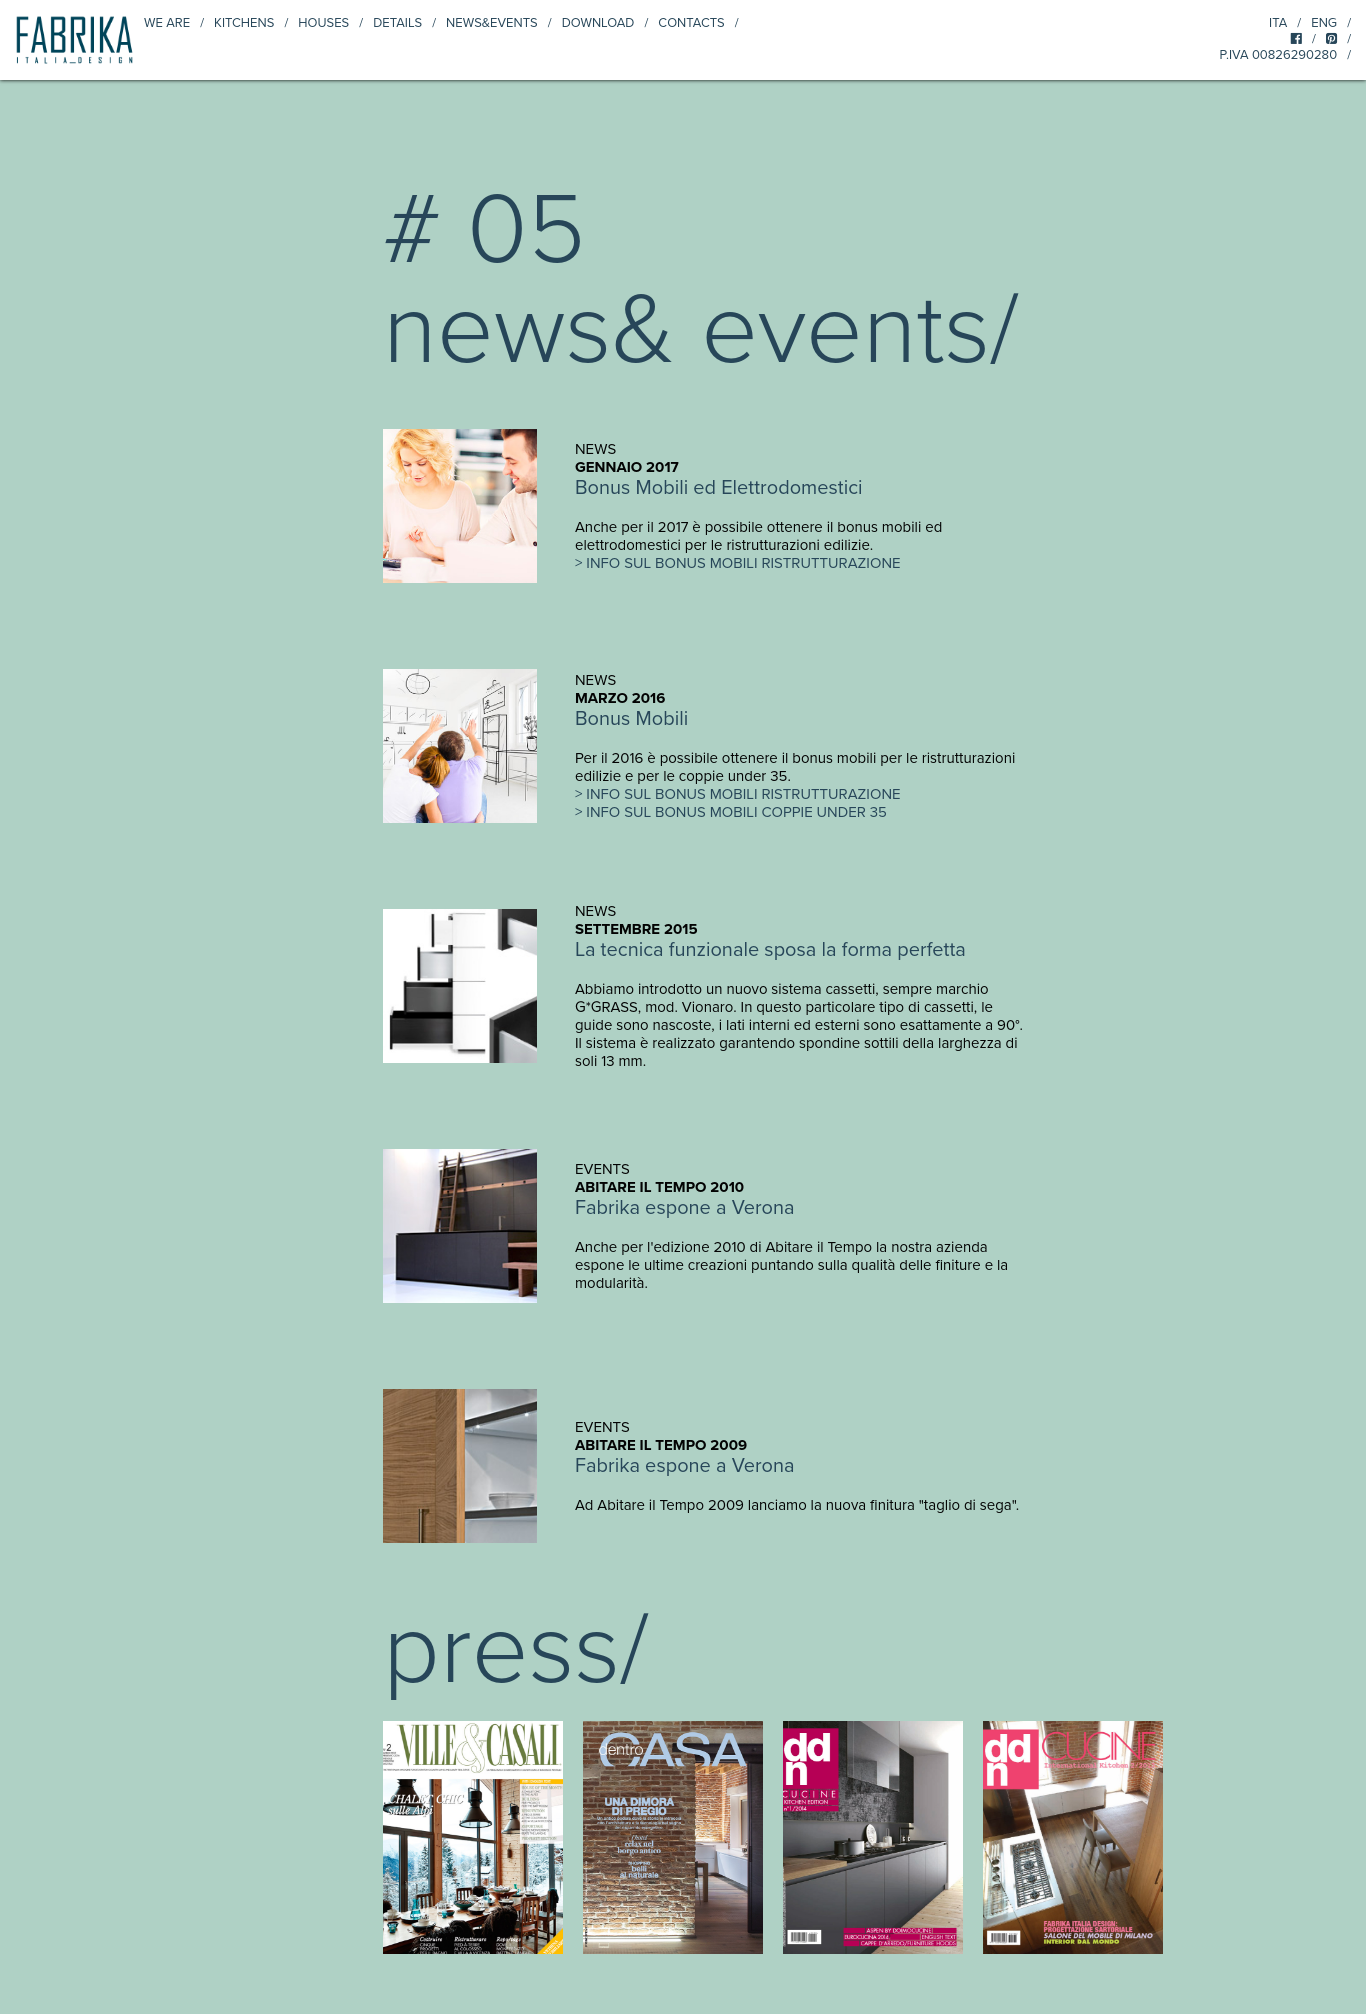
\includegraphics[width=\textwidth]{img/News.png}
            \caption{Pagina News - News.png - (\url{http://www.fabrikaitaliadesign.it/news.html}(2017/06/29))}
        \end{figure}
        Solito problema dell'inspiegabile titolo della pagina enorme che invade tutta la zona di maggior rilevanza e attenzione da parte dell utente infatti in un singolo scroll è possibile visualizzare solo una notizia.\\
        Bene la data per ogni notizia anche se troppo imprecisa, sarebbe stato meglio inserire anche il giorno. Ottima e concisa la descrizione per ogni notizia.\\
        Decisamente troppo spazio vuoto sprecato infatti in 3.7 scroll si ha pochissime informazioni rispetto allo spazio occupato.

\end{document}
